\documentclass{beamer}
\usepackage[ngerman]{babel}
\usepackage[ansinew]{inputenc}
\usepackage{csquotes}
\usepackage{url}
\usepackage{graphicx}
\usepackage{amsmath}
\usepackage{amssymb}
\usepackage{nicefrac}
\usepackage{eurosym}
\usepackage{xcolor}
\usepackage{alltt}
\usepackage{tikz}
\usepackage{ragged2e} 
\usepackage{tabu}
\usetikzlibrary{trees}
\usepackage{calc,color,colortbl,nicefrac}
\newtheorem*{bem}{Bemerkung}
\usepackage{multirow}


%smaller footnotes
\renewcommand{\footnotesize}{\tiny}
%reduce spacing in footnotes
\setlength{\footnotesep}{0em}

%use for inline citation formatting
\newcommand{\textct}[1]{{\textsuperscript{\tiny \color{gray}#1}}}

\newlength{\myX}
\newlength{\myY}

%absolute figure positioning
\usepackage[absolute,overlay]{textpos}
  \setlength{\TPHorizModule}{1mm}
  \setlength{\TPVertModule}{1mm}

%quote environment with reference 
\def\signed #1{{\leavevmode\unskip\nobreak\hfil\penalty50\hskip2em
  \hbox{}\nobreak\hfil(#1)%
  \parfillskip=0pt \finalhyphendemerits=0 \endgraf}}
\newsavebox\mybox
\newenvironment{aquote}[1]
  {\savebox\mybox{#1}\begin{quote}}
  {\signed{\usebox\mybox}\end{quote}}

\definecolor{purp}{HTML}{3333b3}
\definecolor{dgrey}{rgb}{0.8,0.8,0.8}
\definecolor{bgrey}{rgb}{0.95,0.95,0.95}

\usepackage{graphicx}
\graphicspath{{img/}}

\newlength{\stdlength}
% Standardlaenge fuer Skript und Folien
\setlength{\stdlength}{8cm}

\usetheme{Copenhagen}
\usefonttheme{professionalfonts}
\usecolortheme{default}

\bibliography{literature}
\usepackage[style=authoryear, backend=bibtex]{biblatex} 
\addbibresource{literature.bib}

\defbibenvironment{bibliography}
{\list{}
{\setlength{\leftmargin}{\bibhang}%
\setlength{\itemindent}{-\leftmargin}%
\setlength{\itemsep}{6px}%
\setlength{\parsep}{\bibparsep}}}
{\endlist}
{\item \scriptsize}

\definecolor{mygrey}{RGB}{80,80,80}

\setbeamertemplate{headline}
{%
\hfill
\textbf{\insertsection} \
\insertsubsection \
\insertframenumber / \inserttotalframenumber
}
\setbeamertemplate{navigation symbols}{}

\title{Krankheitsausbreitung in Bienenpopulationen}
\author{
S. B�r, D. Haake, F. Rosner
}

\institute{
Martin-Luther-Universit�t Halle-Wittenberg
}
\date{16. Juli 2013}

\begin{document}

\frame{\titlepage 
\parbox{0cm}{\tiny 
\vspace{-30pt}\color{mygrey}
\begin{tabbing}
XXXXXXXXXXXXXXXXXXXXXX\=XXXXXXXXXXX\= \kill \\
\>Veranstaltung:\> "`Simulation: Techniken und Software"'\\
\\
\>Dozenten:\> Prof. Dr. Taieb Mellouli \\
\>\> Michael R�mer
\end{tabbing}
}
}

\begin{frame}
\frametitle{Gliederung}
\tableofcontents
\end{frame}

\section{Zielstellung}
\frame{\frametitle{Gliederung} \tableofcontents[currentsection]}

\begin{frame}{Zielstellung}
\textbf{Problemstellung}
\begin{itemize}
\item Bienen k�nnen sich mit einer Krankheit infizieren
\item erkrankte Bienen k�nnen Krankheit kompletten Bienenstock anstecken
\item dies kann zum Absterben eines Stocks f�hren
\end{itemize}

\vspace*{1em}

\textbf{Zielstellung}
\begin{itemize}
\item daher soll Einfluss der Bienenstockplatzierung auf Ausbreitungsgeschwindigkeit der Krankheit innerhalb der Bienenpopulation untersucht werden
\end{itemize}

\end{frame}

\section{Problemabgrenzung, Daten und Annahmen}

\subsection{Problemabgrenzung}
\frame{\frametitle{Gliederung} \tableofcontents[currentsubsection]}

\begin{frame}
\frametitle{Problemabgrenzung (1)}
\begin{itemize}
\item Imker besitzen eine bestimmte Anzahl Bienenst�cke, die auf einer festgelegten Fl�che platziert werden sollen
\item eine Bienenk�nigin legt solange Eier bis Kapazit�t ihres Stocks erreicht ist
\item Bienen fliegen zu Bl�ten, sammeln Nektar, bringen diesen zur�ck und ruhen sich aus
\item Bienen sterben entweder eines nat�rlichen Todes oder durch die Krankheit
\item erkrankte Bienen k�nnen vor Ablauf der Inkubationszeit andere Bienen anstecken
\end{itemize}
\end{frame}

\begin{frame}
\frametitle{Problemabgrenzung (2)}
\begin{itemize}
\item eine erkrankte Biene kann weitere Bienen im Stock oder an Bl�ten anstecken
\item sobald eine Biene Symptome zeigt, wird sie vom Stock ausgesto�en, fliegt ziellos umher und stirbt nach kurzer Zeit ohne weitere Bienen anzustecken % Annahme von uns??
\item Bienen k�nnen versehentlich zu einem falschen Stock fliegen
	\begin{itemize}
	\item nachdem sie dort ihren Nektar abgegeben haben, werden sie aus dem Stock entfernt
	\item w�hrend des Aufenthalts k�nnen andere Bienen angesteckt werden
	\end{itemize}
\end{itemize}
\end{frame}

\subsection{Annahmen}
\frame{\frametitle{Gliederung} \tableofcontents[currentsubsection]}

\begin{frame}
\frametitle{Annahmen}
\begin{itemize}
\item in Natur werden verschiedenen Bienen, verschiedene Aufgaben zugeteilt (Bienenstock umsorgen, Nektar sammeln)
\begin{itemize}
\item[$\Rightarrow$] 
 im Modell wird darauf verzichtet und es befindet sich immer ein bestimmter Anteil im Stock
\end{itemize}
\item ein bestimmter Prozentsatz Bienen ist am Anfang der Simulation bereits erkrankt
\end{itemize}
\bigskip
\footnotesize\cite[Vgl.][]{tautz2007phaenomen} \\
\footnotesize\cite[Vgl.][]{genersch2010honey} \\
\footnotesize\cite[Vgl.][]{tautz2013bee} \\
\end{frame}

\subsection{Eingabedaten}
\frame{\frametitle{Gliederung} \tableofcontents[currentsubsection]}

\begin{frame}
\frametitle{Eingabedaten}
\begin{itemize}
\item verf�gbare Anbaufl�che und maximale Anzahl Bienenst�cke des Imkers
\item Lebensdauer, Tragekapazit�t, Fluggeschwindigkeit einer Biene
\item Nektarmenge und Regenerationsdauer einer Bl�te
\item Verweildauer einer Biene im eigenen/fremden Stock
\item Wahrscheinlichkeit f�r Verfliegen zu fremdem Stock
\item Eierlegerate einer K�nigin und Kapazit�t eines Bienenstocks
\item Anteil der Sammler im Stock
\item Anteil initial erkrankter Bienen
\item Inkubationszeit und Ansteckungswahrscheinlichkeit f�r gesunde Bienen
\end{itemize}
\bigskip
\footcite[Vgl.][]{tautz2007phaenomen} \\
\footnotesize\cite[Vgl.][]{genersch2010honey} \\
\footnotesize\cite[Vgl.][]{tautz2013bee} \\
\end{frame}

\subsection{Ziel- und Stellgr��e}
\frame{\frametitle{Gliederung} \tableofcontents[currentsubsection]}

\begin{frame}
\frametitle{Ziel- und Stellgr��e}
\textbf{Zielgr��e}
\begin{itemize}
\item Zeitdauer bis komplette Bienenpopulation kollabiert\\
\item[$\Rightarrow$]  Maximierungsproblem
\end{itemize}
\vspace*{1em}
\textbf{Stellgr��e}
\begin{itemize}
\item Anzahl Bienenst�cke und deren Positionierung auf der verf�gbaren Fl�che
\end{itemize}
\end{frame}

\section{Demonstration}
\frame{\frametitle{Gliederung} \tableofcontents[currentsection]}
\begin{frame}
\frametitle{Demonstration}
\textbf{Demo Konfiguration:}
\vspace*{1em}
\begin{itemize}
\item Anzahl der Bienenst�cke: 3 Gruppen mit jeweils einem Stock
\item Anzahl der Bienen pro Stock: 25
\item Anzahl der Blumen: 200
\item Anteil initial erkrankter Bienen: 2\%
\item Infektionswahrscheinlichkeit: 1\%

\end{itemize}
\end{frame}

\begin{frame}
\frametitle{Demonstration}
\textbf{Report Beispiel(1):}
\vspace*{1em}
\begin{center}
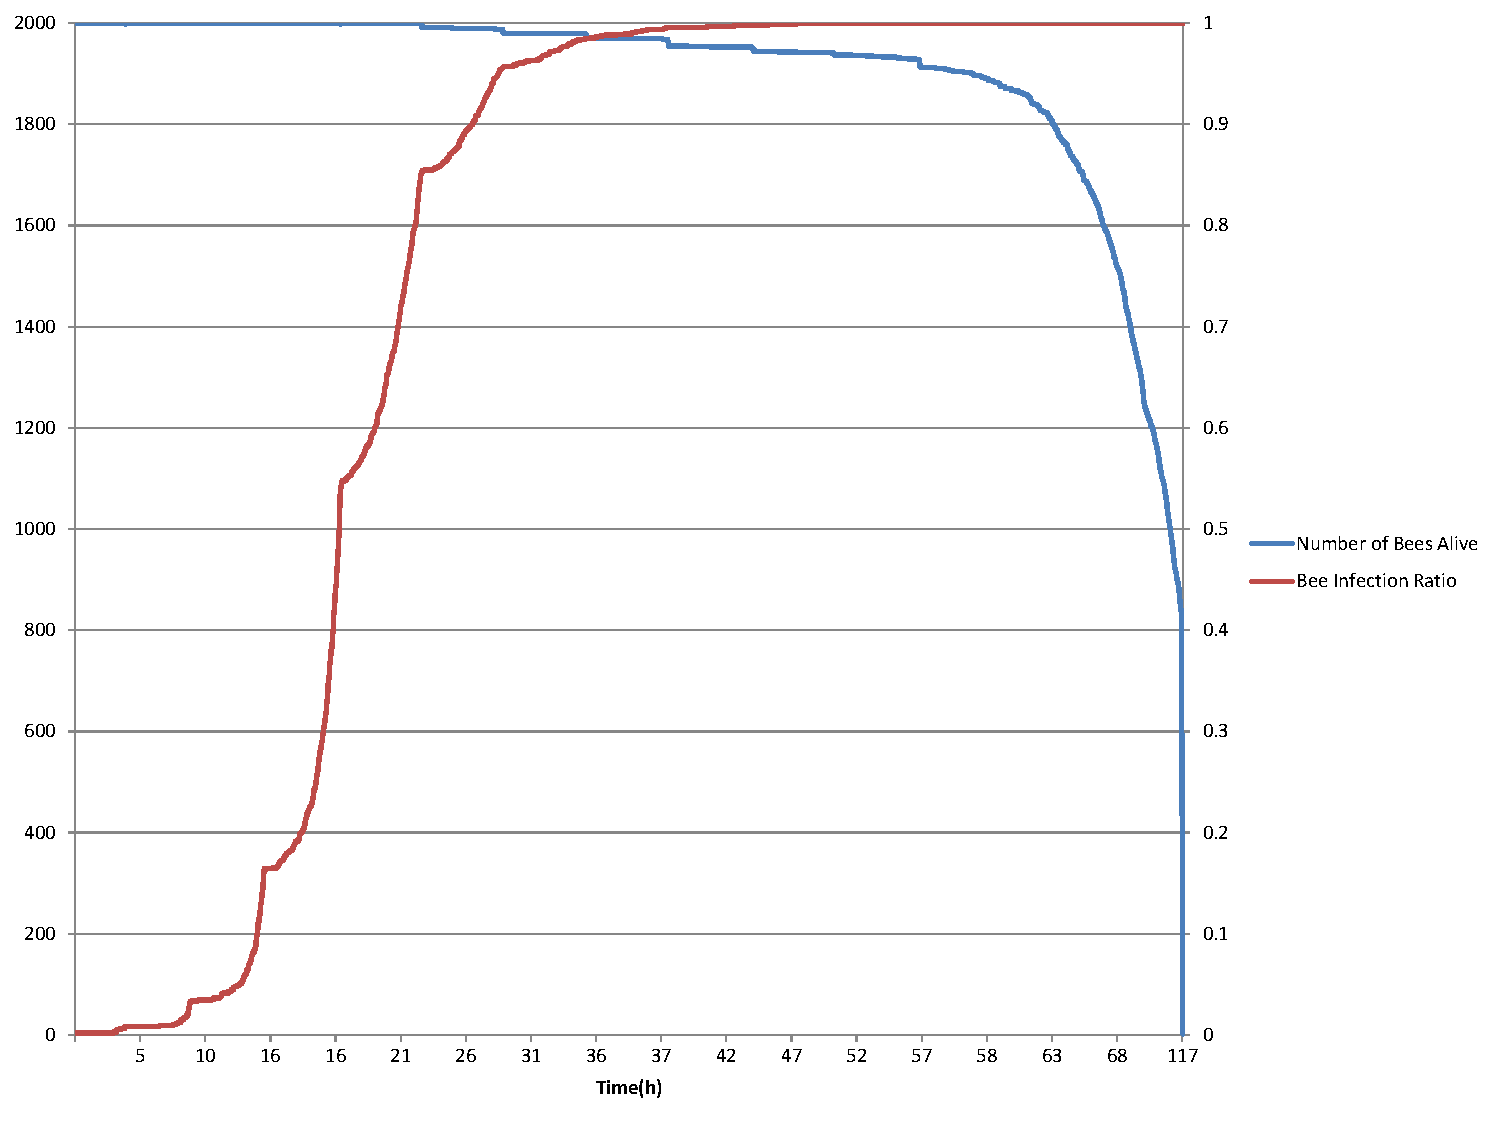
\includegraphics[width=9cm]{bee1.pdf}
\end{center}
\end{frame}

\begin{frame}
\frametitle{Demonstration}
\textbf{Report Beispiel(2):}
\vspace*{1em}
\begin{center}
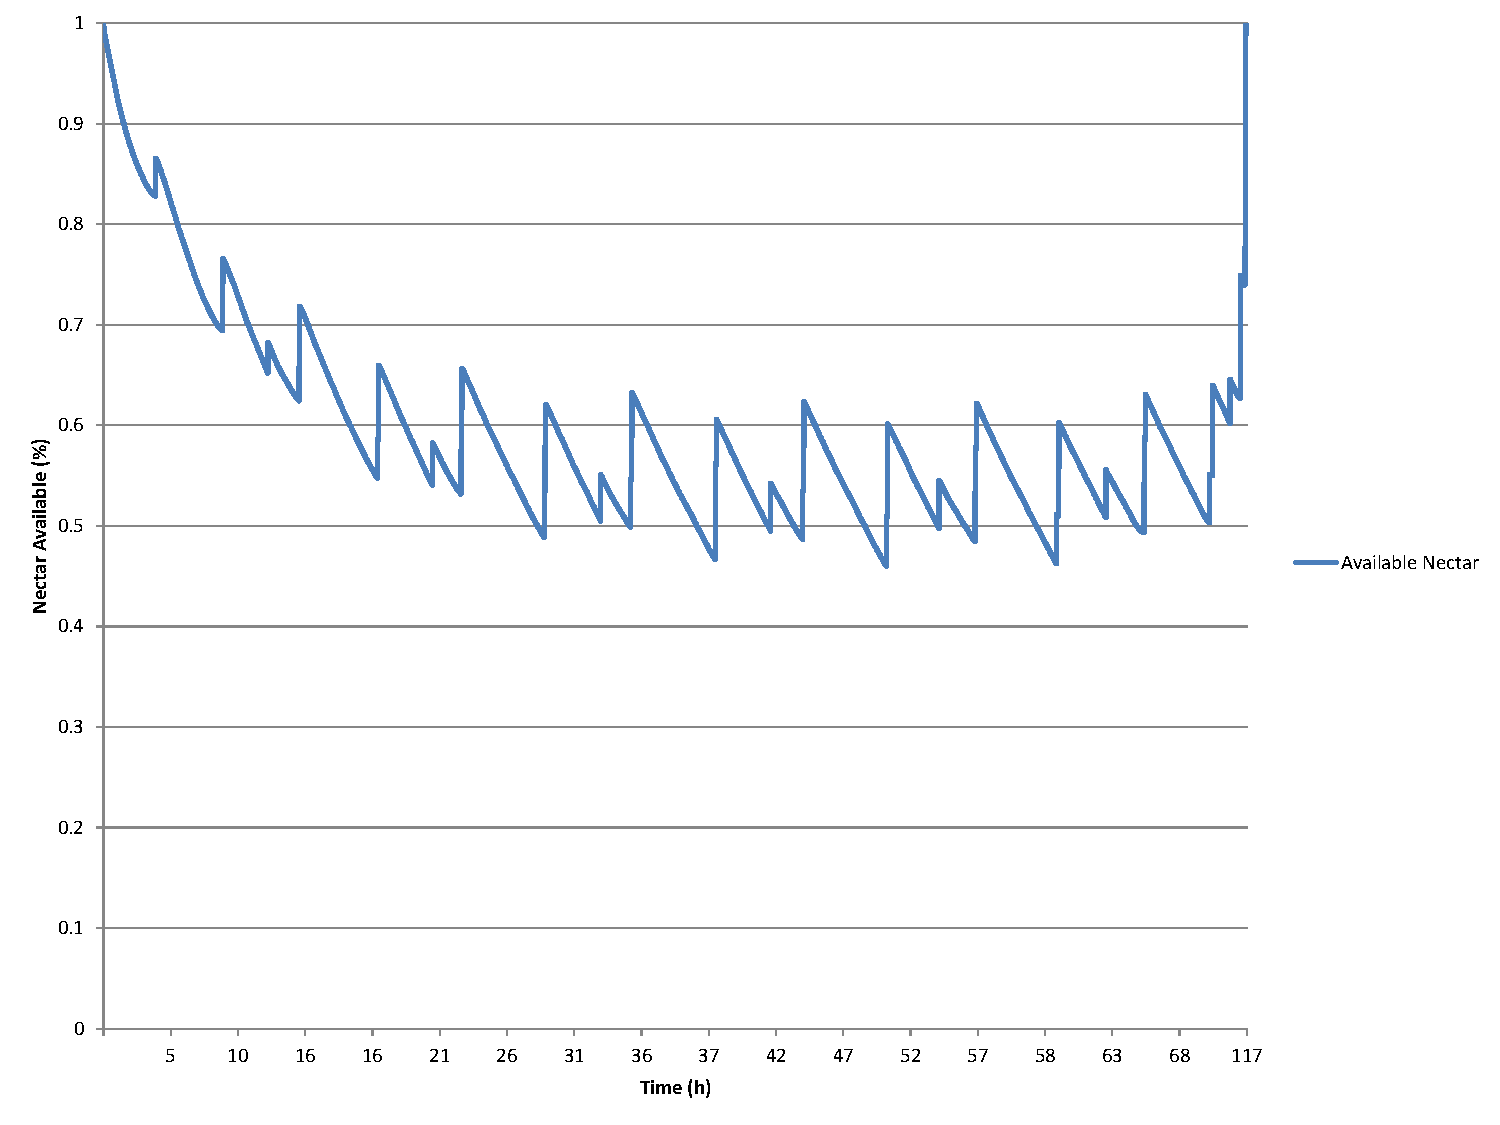
\includegraphics[width=9cm]{bee2.pdf}
\end{center}
\end{frame}

\section{Ergebnisse der Simulation}
\frame{\frametitle{Gliederung} \tableofcontents[currentsection]}
\begin{frame}
\frametitle{Erg}
\end{frame}

\section{Fazit}
\frame{\frametitle{Gliederung} \tableofcontents[currentsection]}
\begin{frame}
\frametitle{Fazit}
\end{frame}


% cite all resources to be printed in bibliography
% this frame will not be shown
\begin{frame}<0>
\frametitle{Quellen}

\end{frame}

\begin{frame}
\thispagestyle{empty}
\begin{center}
\Huge
Vielen Dank f�r Ihre Aufmerksamkeit!\\
\ 
\\
Fragen?
\end{center}
\end{frame}

\end{document}